\documentclass[t]{beamer}
\usetheme[height=7mm]{Rochester}
\setbeamercovered{transparent}
\setbeamertemplate{navigation symbols}{}
%\setbeamertemplate{footline}[frame number]
\setbeamertemplate{footline}
{
\leavevmode%
  \hbox{%
  \begin{beamercolorbox}[wd=\paperwidth,dp=2.5ex,ht=3ex]{}%
    \hspace*{2em}%
    {\hfill Folie \insertframenumber}%
    \hspace*{2em}%
  \end{beamercolorbox}%
  }%
}

\usepackage[german]{babel}
\usepackage[utf8]{inputenc}
\usepackage[vlined]{algorithm2e}
\usepackage{adjustbox}
\DontPrintSemicolon

\theoremstyle{plain}
\newtheorem{Korollar}{Korollar}


\title[Treaps]{Randomisierte Suchstrukturen: Treaps}
\author[M. Beck, R. McDaniel]{Moritz Beck, Robert McDaniel}
\date[10.06.2015]{10. Juni 2015}


\AtBeginSection[]{
    {\setbeamertemplate{footline}{}
    \begin{frame}<beamer>{Gliederung}
        \tableofcontents[currentsection]
    \end{frame}}
}
\AtBeginSubsection[]{
    {\setbeamertemplate{footline}{}
    \begin{frame}<beamer>{Gliederung}
        \tableofcontents[currentsubsection]
    \end{frame}}
}

\beamerdefaultoverlayspecification{<+->}

\begin{document}

{
\setbeamertemplate{footline}{}

\begin{frame}%[plain]
    \titlepage
\end{frame}

\begin{frame}{Gliederung}
    \tableofcontents
\end{frame}
}

\section{Einführung und Motivation}
\subsection{Grundmotivation}
\begin{frame}{Grundmotivation}
    Gesucht: Möglichst schnelle Datenstruktur mit Unterstützung folgender Methoden:
    \bigskip
    \begin{itemize}
        \item<2-> $S$ = MakeSet()
        \item<3-> Insert($i, S$)
        \item<4-> Delete($k, S$)
        \item<5-> Find($k, S$)
        \item<6-> $S$ = Join$(S_1, i, S_2)$
        \item<7-> $S$ = Merge$(S_1, S_2)$
        \item<8-> $S_1, S_2$ = Split$(k, S)$ 
    \end{itemize}
    \bigskip
    \onslide<9-> Bereits bekannt: Binäre Suchbäume
\end{frame}

\subsection{Laufzeiten bei binären Suchbäumen}
\begin{frame}{Laufzeiten bei binären Suchbäumen}
    \setbeamercovered{invisible}
    \begin{table}
    	\resizebox{7 cm}{!}{
        \begin{tabular}{l | c }
        Methode & Laufzeit\\
        \hline
        \visible<2->{$S$ = MakeSet()} & \only<2->{$O(1)$}\\
        \visible<3->{Insert$(i, S)$} & \only<3->{$O(h)$} \\
        \visible<4-> {Delete$(k, S)$} &
        \visible<4-> {$O(h)$} \\
        \visible<5-> {Find$(k, S)$} &
        \visible<5-> {$O(h)$} \\
        \visible<6-> {$S$ = Join($S_1, i, S_2$)} &
        \visible<6-> {$O(1)$} \\
        \visible<7-> {$S$ = Merge($S_1, S_2$)} & \only<7-> {$O(h_1)$} \\
        \visible<8-> {$S_1, S_2$ = Split$(k, S)$} & \only<8-> {$O(h)$}
        \end{tabular}
        }
    \end{table}
    \begin{itemize}
        \item\onslide<3->$h$ = Höhe des Baums
        \item\onslide<7->$h_1$ = Höhe des ersten Baums
    \end{itemize}
\end{frame}

\subsection{Probleme bei binären Suchbäumen}
    \begin{frame}{Probleme bei binären Suchbäumen}
    \begin{itemize}
    \item Es zeichnet sich ab: Hohe Abhängigkeit von Höhe des Baums $\Rightarrow$ Schwanken zwischen $O(\log(n))$ und $O(n)$
    \item Problem: Binärbäume sind oft unoptimal und extreme Fälle führen zu langen Laufzeiten!
    \end{itemize}
    {\only<3->{\hspace{1.1 in}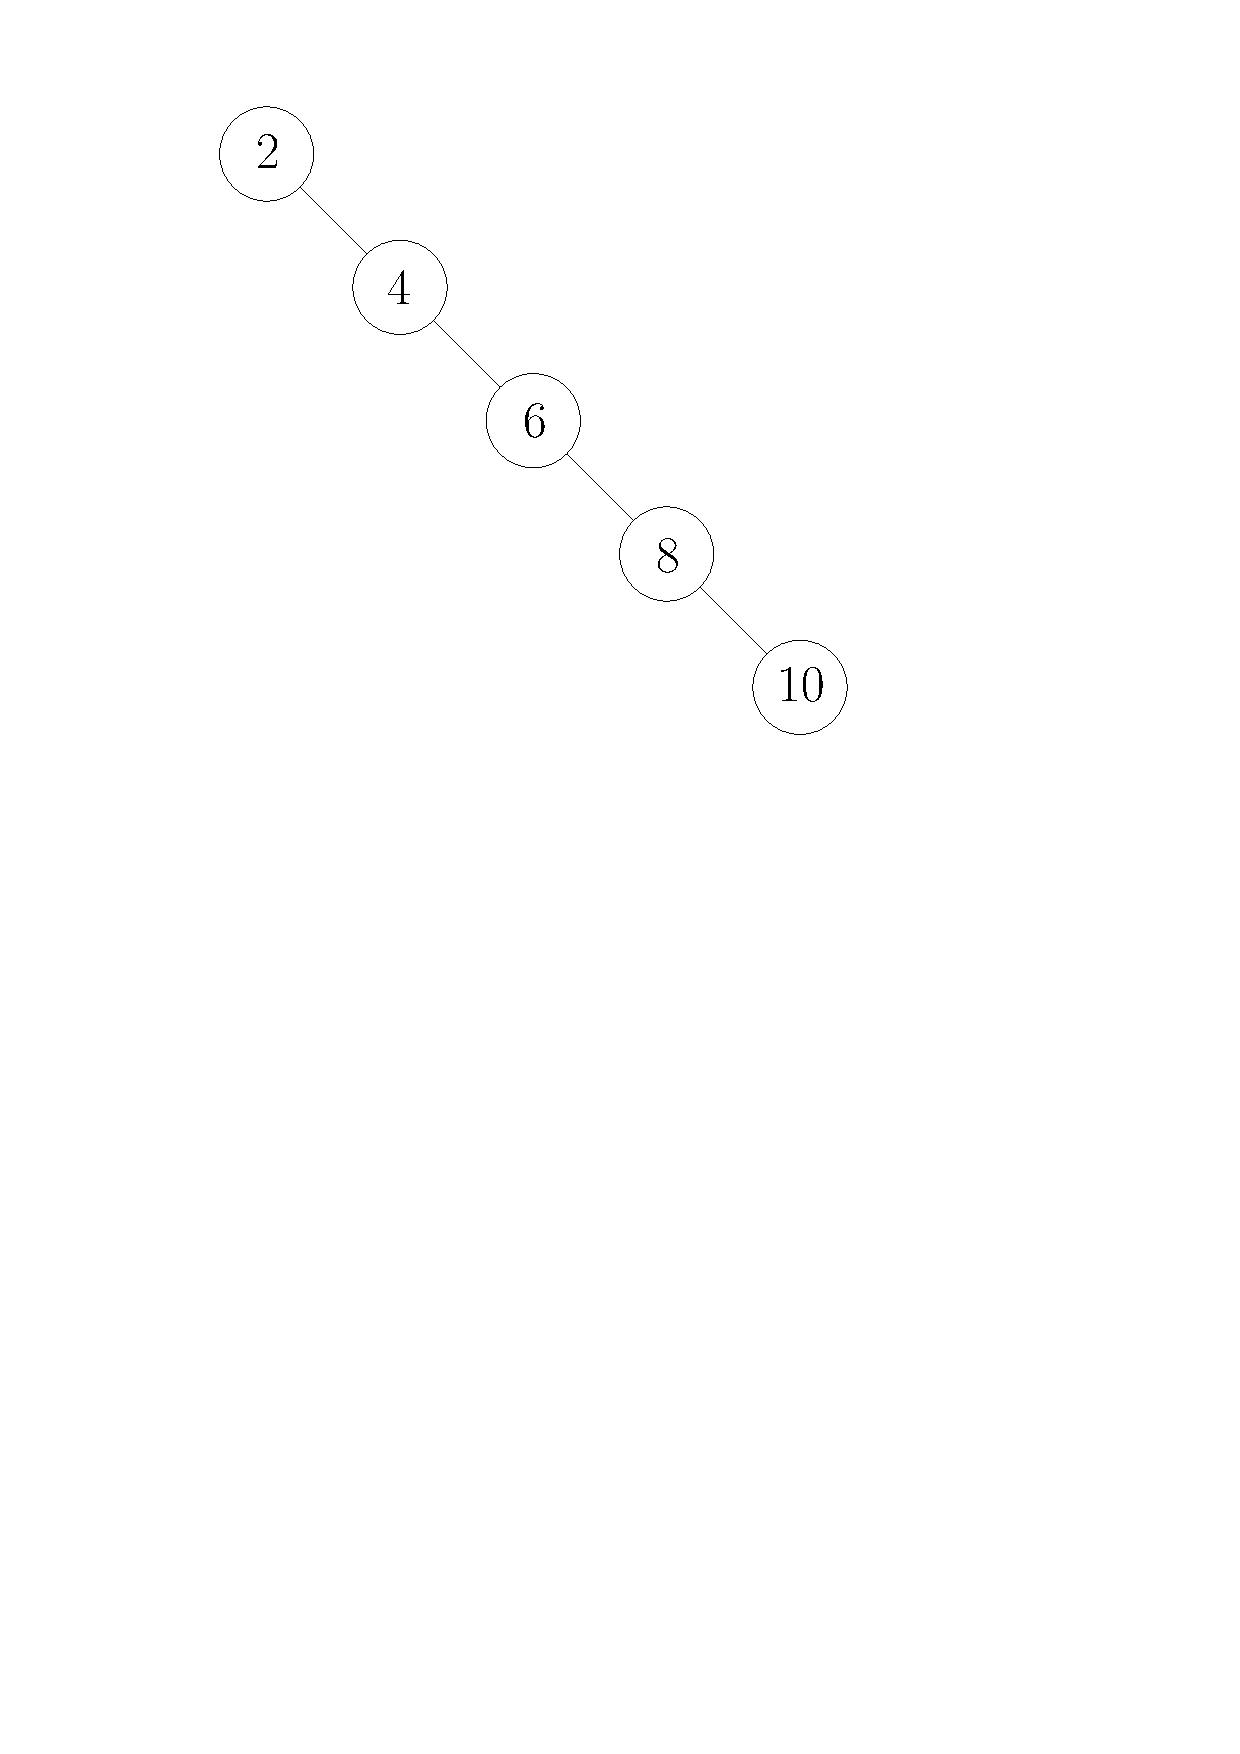
\includegraphics[width=.5\textwidth] {img/BinaryTree.pdf}}}
\end{frame}

\begin{frame}{Probleme bei binären Suchbäumen}
    \begin{itemize}
    \item Problem: Hohe worst-case-Laufzeiten
    \item Lösung: Vorherige Optimierung (Balancieren)?
    \item Balancieren bringt neue Probleme:
        \begin{itemize}
        \item Erhöhter Overhead
        \item Höhere Laufzeiten durch konstantes Updating
        \item Speichern von zusätzlicher Information möglicherweise notwendig
        \end{itemize}
    \bigskip
    \item Lösungsidee: Balancieren durch Randomisieren?
    \begin{itemize}
        \item Einfache Implementierung
        \item Keine weitere Information zu speichern
        \item Schnelle Ausführung
    \end{itemize}
\end{itemize}
\end{frame}


\section{Treaps}
\subsection{Grundlagen}
\begin{frame}{Treaps - Definition}
    \begin{center}
        \color{red}{Binary \textbf{Tr}ee} + \color{blue}{H\textbf{eap}} = \textbf{\textcolor{red}{Tr}\textcolor{blue}{eap}}
    \end{center}
    \begin{itemize}
        \item<2-> \textcolor{red}{Schlüssel}
        \item<3-> \textcolor{blue}{Priorität} (meist Implementierungsdetail)
    \end{itemize}
    \vspace{1em}
    \hfill\only<4->{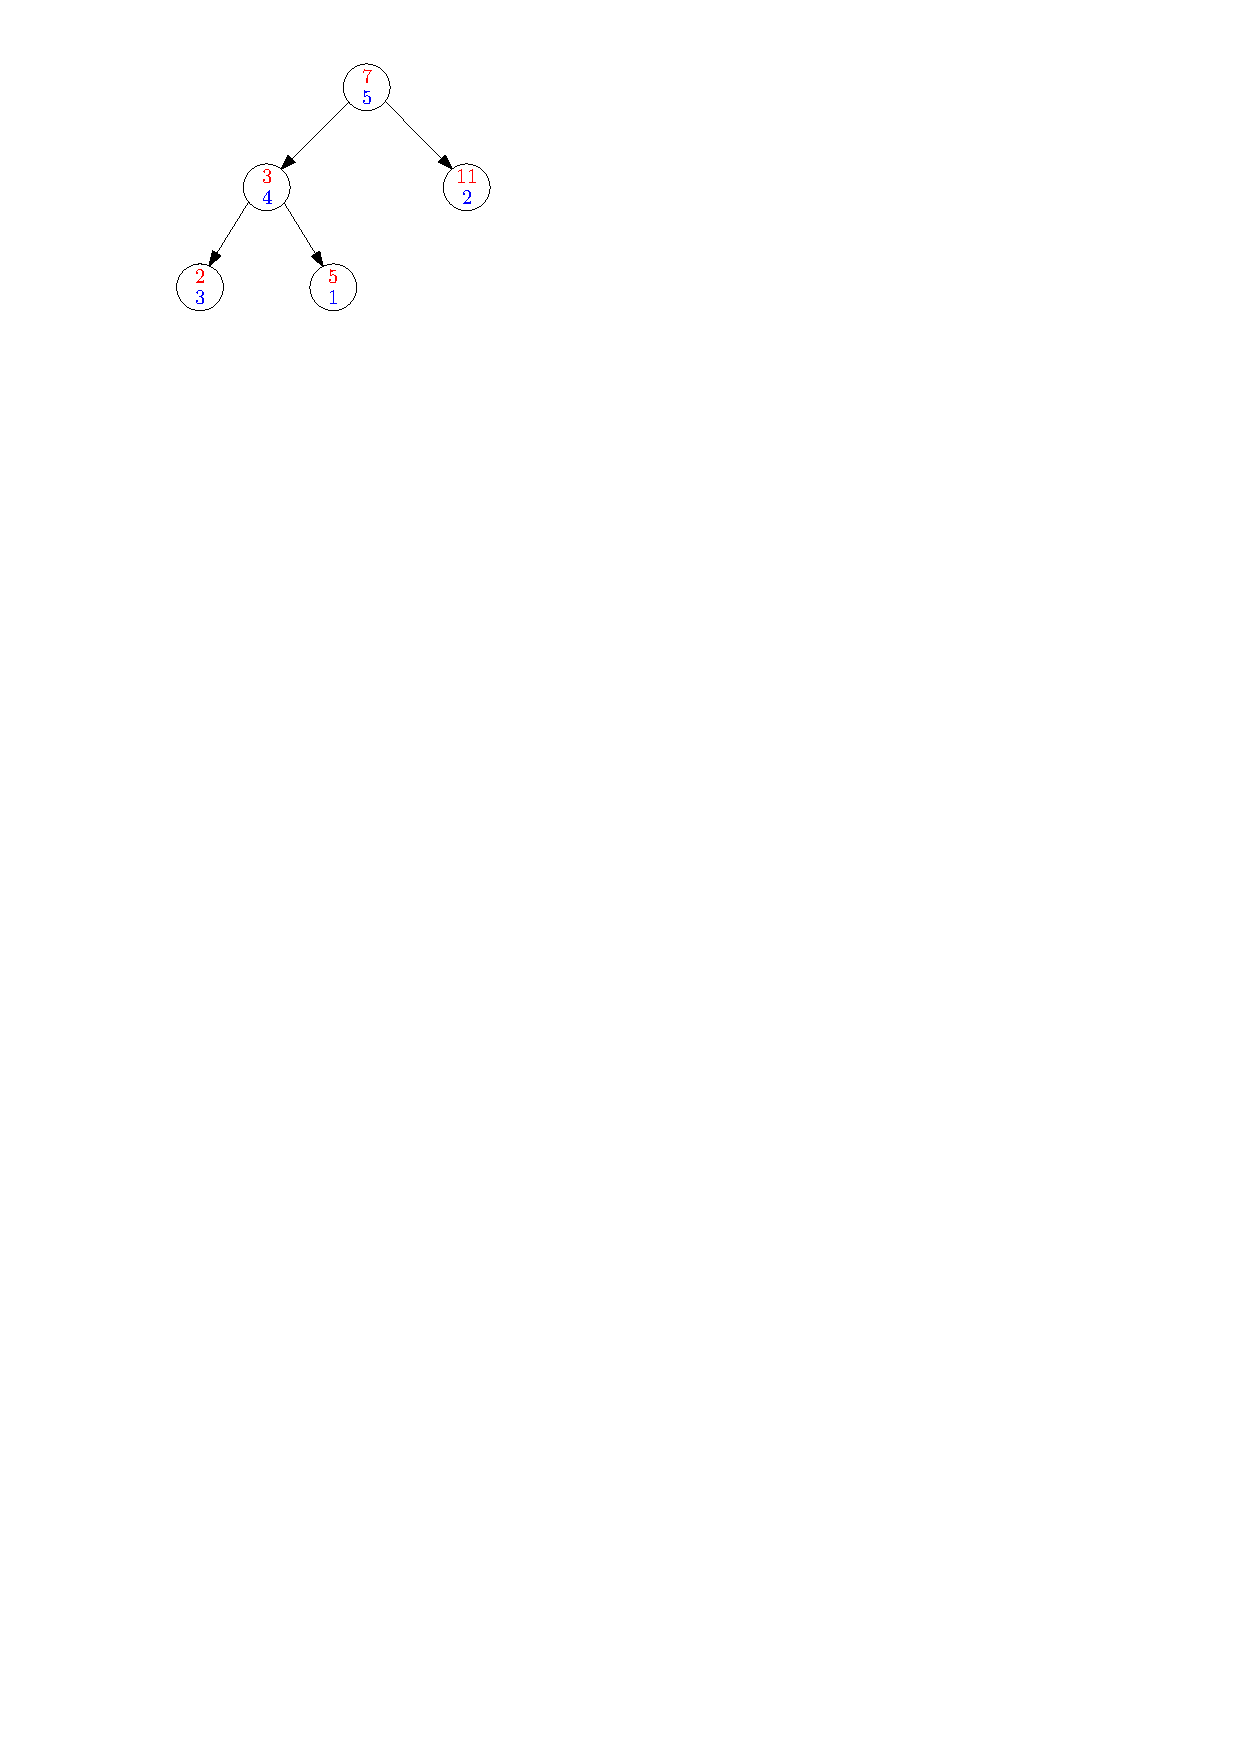
\includegraphics[page=1,width=.5\textwidth]{img/Beispiel_Treap.pdf}}
\end{frame}

\subsection{Existenz eindeutiger Treaps}
\begin{frame}{Existenz eindeutiger Treaps}
    \begin{Satz}
        Für jede Menge $S = \{(k_1,p_1), \dots, (k_n, p_n)\}$ von Schlüssel-Priorität-Paaren mit paarweise unterschiedlichen Schlüsseln und Prioritäten existiert genau ein gültiger Treap.
    \end{Satz}
    \only<2-5>{
    \begin{proof}
        Per Induktion über $n = \left|S\right|$:
        \raisebox{3em}{
        \begin{columns}<2->
        \begin{column}[t]{.65\textwidth}
            \begin{itemize}
            \item<3-> \textbf{IA}: n = 0: \\ leere Menge $\leftrightarrow$ leerer Baum \textcolor[rgb]{0,.7,0}{\Large\checkmark}
            \item<4-> \textbf{IS}: $t   = \{(k_t, p_t) \in S \mid p_t \text{ maximal}\}$
                                   $M_< = \{(k_i, p_i) \in S \mid k_i < k_t\}$ \\
                                   $M_> = \{(k_i, p_i) \in S \mid k_i > k_t\}$
            \end{itemize}
        \end{column}
        \begin{column}[t]{0.35\textwidth}
            \raisebox{-\totalheight}{\visible<5->{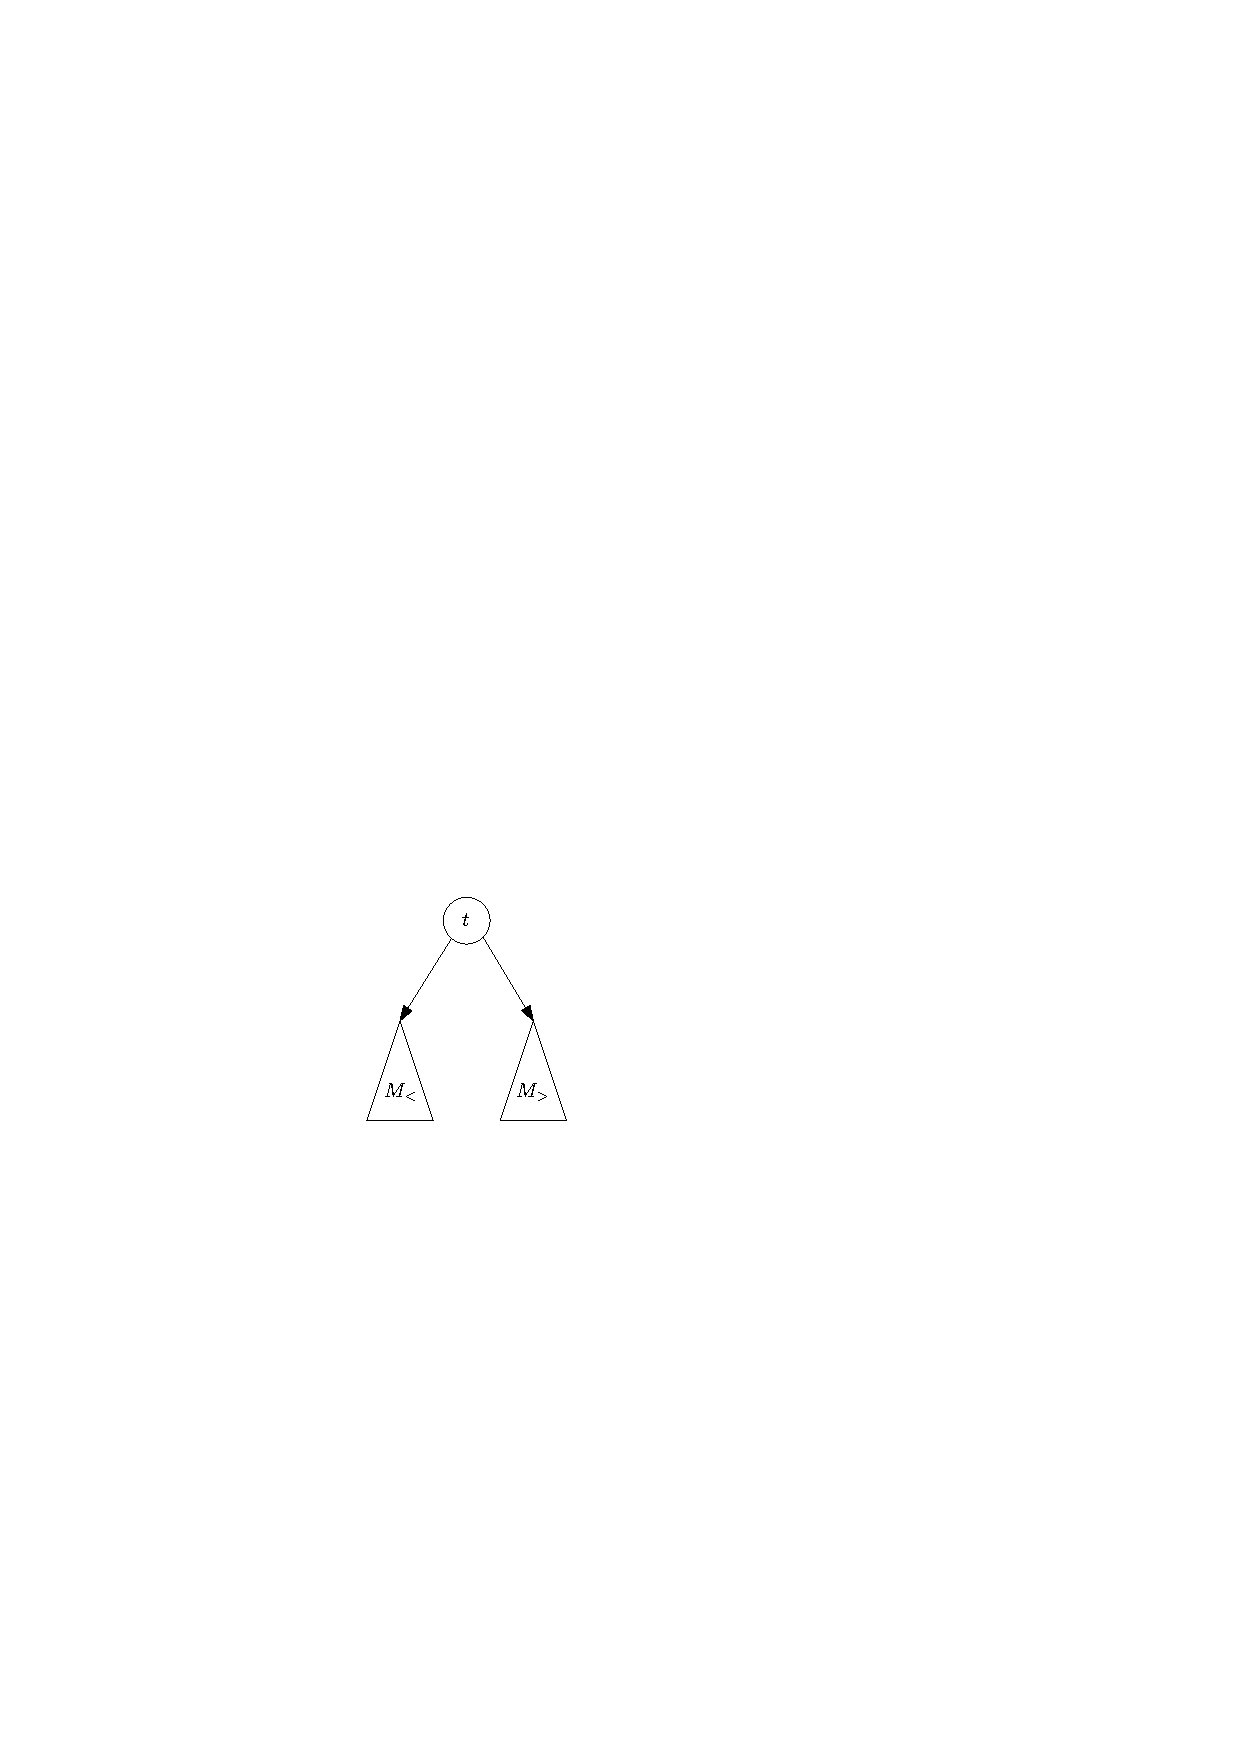
\includegraphics[width=.9\textwidth]{img/Eindeutigkeit_IS.pdf}}}
        \end{column}
        \end{columns}}
    \end{proof}}
    \visible<6->{\begin{Folgerung}
        Die Reihenfolge, in der Knoten eingefügt oder gelöscht werden, ist für die Struktur eines Treaps irrelevant.
    \end{Folgerung}}
\end{frame}

\subsection{Implementierung}
\begin{frame}{Rotation}
    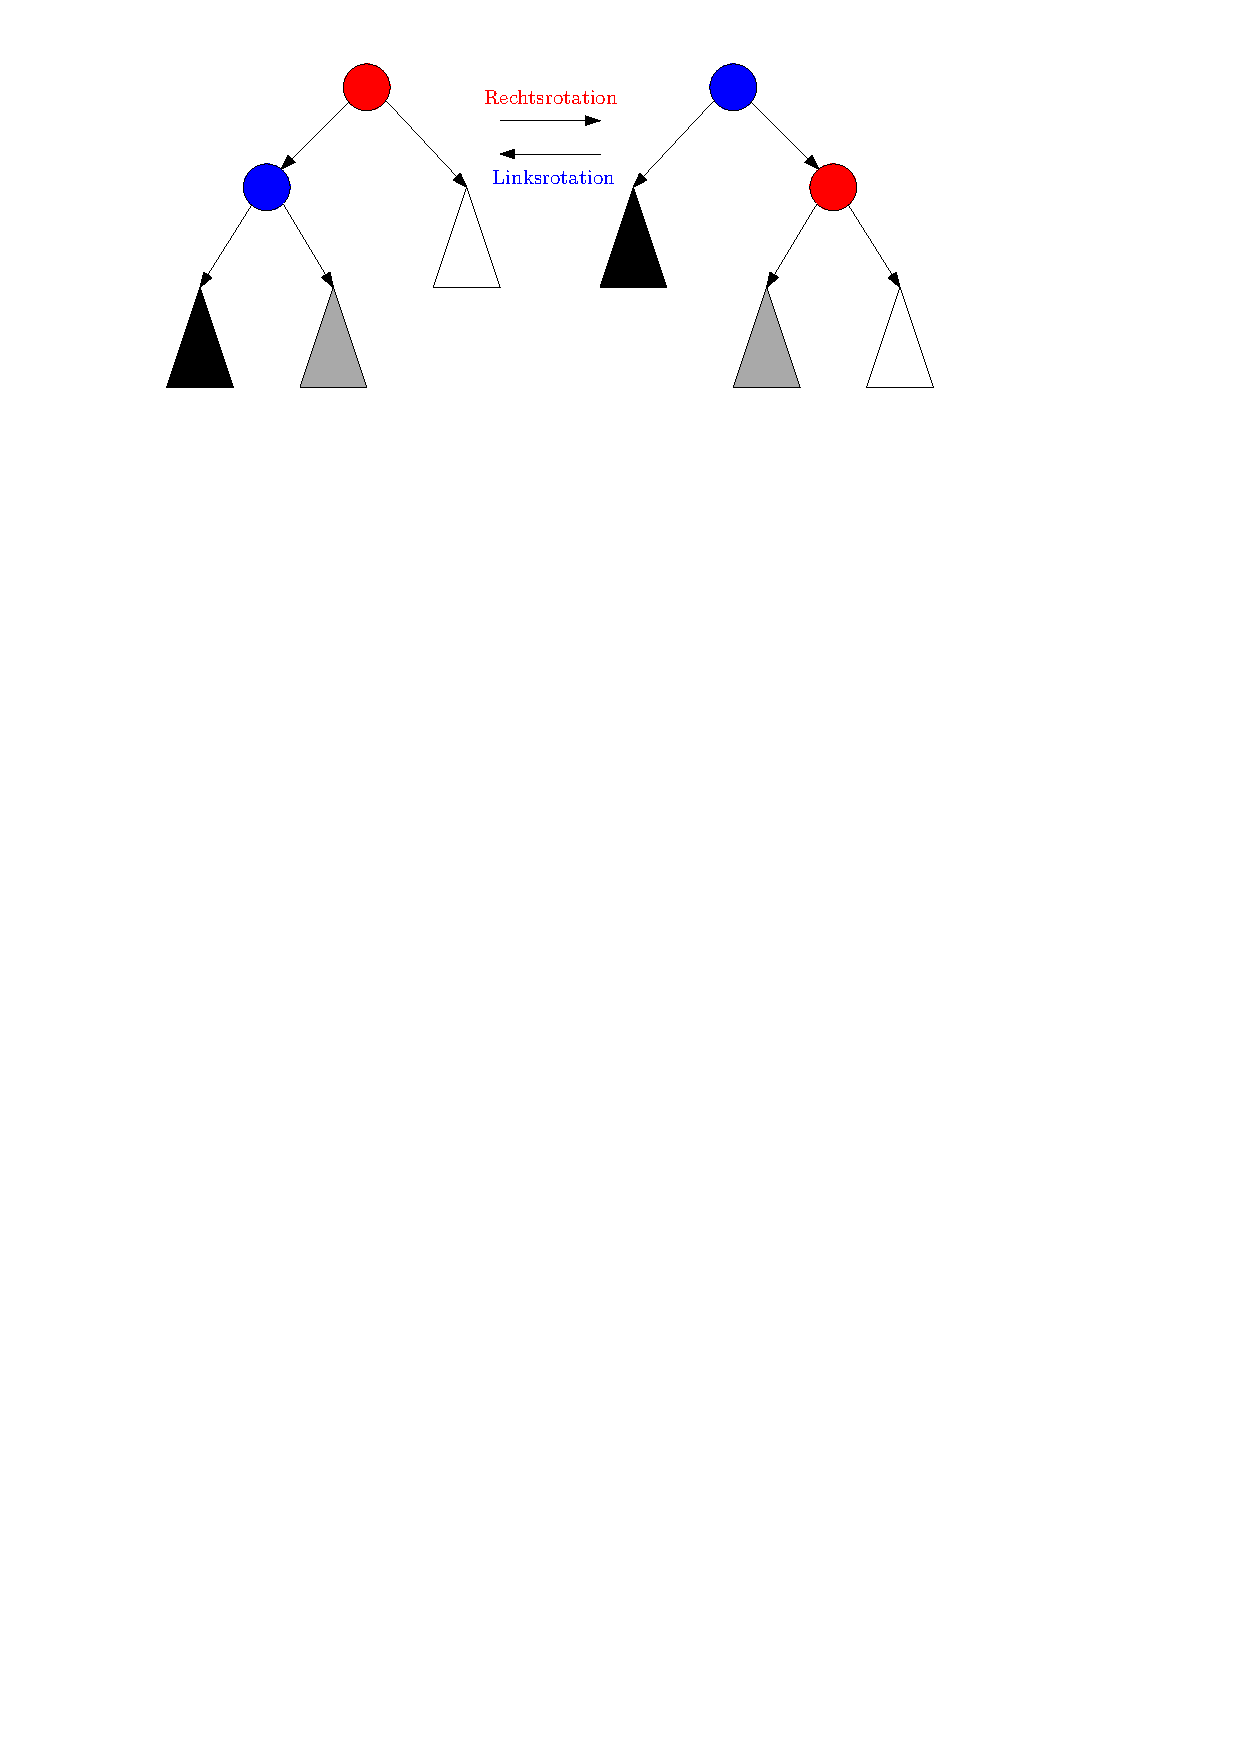
\includegraphics[width=\textwidth]{img/Tree_Rotation_color.pdf}
    \begin{itemize}
        \item<2-> erhält Suchbaumeigenschaft
        \item<3-> ändert Prioritätenreihenfolge rot/blau
    \end{itemize}
\end{frame}
\begin{frame}{Find + Update}
    \begin{columns}<1->
    \begin{column}{.65\textwidth}<1->
        \begin{itemize}
            \item<1> Find($k$, $S$): Normale Suche in einem Binärbaum
            \item<2> Insert($i$, $S$):
                \begin{algorithm}[H]
                    %\Ein{Knoten $i$, Treap $S$}
                    Füge $i$ als Blatt in $S$ ein \;
                    \While{$i$.parent.prio $<$ $i$.prio}{
                        Rotiere $i$ nach oben \;
                    }
                \end{algorithm}
            \item<3> Delete($k$, $S$):
                \begin{algorithm}[H]
                    \SetKw{Not}{not}
                    \While{\Not istBlatt($i$)}{
                        Rotiere $i$ nach unten \;
                    }
                    Lösche Blatt $i$ aus $S$ \;
                \end{algorithm}
        \end{itemize}
    \end{column}
    \begin{column}{.35\textwidth}<1->
        \raisebox{-\totalheight}{
            \includegraphics<1>[width=.8\textwidth]{img/Impl_Find.pdf}
            \includegraphics<2>[width=.8\textwidth]{img/Impl_Insert.pdf}
            \includegraphics<3>[width=.8\textwidth]{img/Impl_Delete.pdf}
        }
    \end{column}
    \end{columns}
% Insert(i, S) // S wird verändert
% Delete(k, S) // S wird verändert
% Find(k, S)
% S = Join(S_1, i, S_2)
% S = Merge(S_1, S_2)
% S_1, S_2 = Split(k, S)
\end{frame}

\begin{frame}{Mengenoperationen}
    \begin{columns}<1->
    \begin{column}{.65\textwidth}<1->
        \begin{itemize}
            \item<1> Join($S_1$, $i$, $S_2$):
                \begin{algorithm}[H]
                    \SetKw{Or}{or}
                    $i$.left $\gets S_1$ \;
                    $i$.right $\gets S_2$ \;
                    \While{$i$.prio $<$ $i$.left.prio\\ \Or $i$.prio $<$ $i$.right.prio}{
                        Rotiere $i$ nach unten \;
                    }
                    \Return $i$
                \end{algorithm}
            \item<2> Merge($S_1$, $S_2$):
                \begin{algorithm}[H]
                    $i$ $\gets$ Find($\infty$, $S_1$) \tcp{Maximum}
                    Delete($i$, $S_1$) \;
                    \Return Join($S_1$, $i$, $S_2$) \;
                \end{algorithm}
            \item<3> Split($k$, $S$):
                \begin{algorithm}[H]
                % TODO?
                    \tcp{Übungsaufgabe ;-)}
                \end{algorithm}
        \end{itemize}
    \end{column}
    \begin{column}{.35\textwidth}<1->
        \raisebox{-\totalheight}{
            %\includegraphics<1>[width=.8\textwidth]{img/Impl_Join.pdf} %TODO: Bild fehlt noch
            \includegraphics<1>[width=.8\textwidth]{img/dummy.pdf}
            %\includegraphics<2>[width=.8\textwidth]{img/Impl_Merge.pdf} %TODO: Bild fehlt noch
            \includegraphics<2>[width=.8\textwidth]{img/dummy.pdf}
            %\includegraphics<3>[width=.8\textwidth]{img/Impl_Split.pdf} %TODO: Bild fehlt noch
            \includegraphics<3>[width=.8\textwidth]{img/dummy.pdf}
        }
    \end{column}
    \end{columns}
% Insert(i, S) // S wird verändert
% Delete(k, S) // S wird verändert
% Find(k, S)
% S = Join(S_1, i, S_2)
% S = Merge(S_1, S_2)
% S_1, S_2 = Split(k, S)
\end{frame}
\begin{frame}{Übungsaufgabe -- Implementierung Split}
    Aufgabe: Implementieren Sie Split!
    % TODO
\end{frame}

\subsection{Laufzeitanalyse}
\begin{frame}{Mulmuley Games}
    Gegeben seien folgende disjunkte Mengen:
    \begin{itemize}
        \item Spieler $P$
        \item Zuschauer $B$
        \item Trigger $T$
        \item Stopper $S$ (zählen auch als Spieler)
    \end{itemize}
    \only<+->{$P, S$ total geordnet}

    \only<+->{$\forall p \in P, s \in S:\ p < s$}

    \only<+->{Ziehe zufällige Elemente aus einer Menge $X$ bis ein Stopper gezogen wurde oder die Menge leer ist.}

    \only<+->{Zähle die Anzahl der Spieler, die größer sind als alle vorherigen und nach dem ersten Trigger gezogen wurden.}

    \only<+->{Wert des Spiels: Erwartungswert der Anzahl}
\end{frame}
\begin{frame}{Mulmuley Games}
    Wert des Spiels: Erwartungswert der Anzahl
    \begin{itemize}
        \item Spiel A
        \begin{itemize}
            \item $X = P \cup B$
            \item $A^p = H_p$
        \end{itemize}
        \item Spiel C
        \begin{itemize}
            \item $X = P \cup S \cup B$
            \item $C_s^p = 1 + H_{s+p} - H_s$
        \end{itemize}
        \item Spiel D
        \begin{itemize}
            \item $X = P \cup T \cup B$
            \item $D_t^p = H_p + H_t - H_{p+t}$
        \end{itemize}
        % \item Spiel E % TODO: Spiel E weglassen, da nicht verwendet?
        % \begin{itemize}
            % \item $X = P \cup T \cup S \cup B$
            % \item<14-> $E_{t,s}^p = \frac t{t+s} + (H_{s+p} - H_s) - (H_{t+s+p} - H_{t+s})$
        % \end{itemize}
    \end{itemize}
\end{frame}
\begin{frame}{Laufzeitanalyse}
    Zur Laufzeitanalyse genügt es, Delete($k, S$) zu betrachten.

    \uncover<2->{Laufzeit von Delete($k, S$):}
    \begin{columns}
    \begin{column}{.71\textwidth}
        \begin{itemize}
            \item<3-> Tiefe des Knotens mit Schlüssel $k$\\
            (Suche)
            \item<4-> Länge rechter Grat des linken Teilbaums +\\
            Länge linker Grat des rechten Teilbaums\\
            (nach unten rotieren)
        \end{itemize}
        \vspace{1em}
        \uncover<5->{Sei $X$ die Menge aller Knoten.
        Sei $x$ ein Knoten mit Rang $r$ und $X_\leq$ die Menge aller Knoten mit Schlüssel kleiner/gleich $k_x$.}

        \uncover<6->{Füge die Knoten o.E. nach absteigender Priorität ein.}
    \end{column}
    \begin{column}{.29\textwidth}<1->
        \raisebox{-\totalheight}{
        \includegraphics<2>[page=1,height=.75\textheight]{img/Analyse_Delete.pdf}
        \includegraphics<3>[page=2,height=.75\textheight]{img/Analyse_Delete.pdf}
        \includegraphics<4>[page=3,height=.75\textheight]{img/Analyse_Delete.pdf}
        \includegraphics<5->[page=4,height=.75\textheight]{img/Analyse_Delete.pdf}
    }
    \end{column}
    \end{columns}
\end{frame}
\begin{frame}{Laufzeitanalyse -- Tiefe}
    % Tiefe des Knotens: O(log n)
    \uncover<+->{\textbf{Tiefe des Knotens}}

    \uncover<+->{Die Knoten in $X_\leq$ entlang des Suchpfads von $x$ sind genau die, die beim Einfügen am größten sind.}

    \uncover<+->{$\Rightarrow$ Spiel A mit $P = X_\leq, B = X \setminus X_\leq$ ($|P| = r, |B| = n - r$)}

    \uncover<+->{$\Rightarrow$ Erwarteter Wert: $H_r$}

    \uncover<+->{$\Rightarrow$ Länge des Suchpfads: $H_r + H_{n-r+1} - 1 \in O(\log n)$}

    \vspace{1em}
    \uncover<+->{Beispiel: $k_x = 6$}
    \includegraphics<+>[page=1,width=\textwidth]{./img/Laufzeit_Beweis.pdf}
    \includegraphics<+>[page=2,width=\textwidth]{./img/Laufzeit_Beweis.pdf}
    \includegraphics<+>[page=3,width=\textwidth]{./img/Laufzeit_Beweis.pdf}
    \includegraphics<+>[page=4,width=\textwidth]{./img/Laufzeit_Beweis.pdf}
    \includegraphics<+>[page=5,width=\textwidth]{./img/Laufzeit_Beweis.pdf}
    \includegraphics<+>[page=6,width=\textwidth]{./img/Laufzeit_Beweis.pdf}
    \includegraphics<+>[page=7,width=\textwidth]{./img/Laufzeit_Beweis.pdf}
    \includegraphics<+>[page=8,width=\textwidth]{./img/Laufzeit_Beweis.pdf}
    \includegraphics<+>[page=9,width=\textwidth]{./img/Laufzeit_Beweis.pdf}
    \includegraphics<+>[page=10,width=\textwidth]{./img/Laufzeit_Beweis.pdf}
\end{frame}
\begin{frame}{Laufzeitanalyse -- Rotationen}
    % Länge der Grate < 2
    \uncover<+->{\textbf{Anzahl der Rotationen}}

    \uncover<+->{Mit ähnlichen Argumenten:}

    \uncover<+->{Spiel D mit $P = X\leq \setminus \{x\}, T = \{x\}, B = X \setminus X\leq$}

    \uncover<+->{$\Rightarrow$ Erwarteter Wert: $H_{r-1} + H_1 - H_r = 1 - 1/r$}

    \uncover<+->{$\Rightarrow$ Anzahl der Rotationen: $2 - 1/r - 1/(n-r+1) < 2$}
\end{frame}


\section*{Fazit}
\begin{frame}{Fazit}
    Erwartete Laufzeiten bei Treaps:
    \begin{table}
    	\resizebox{7 cm}{!}{ % TODO: Laufzeiten Binärbaum
        \begin{tabular}{l | c }
        Methode & Laufzeit\\
        \hline
        \visible<+->{Insert$(i, S)$} &
        \only<.->{$O(\log n)$} \\
        \visible<+-> {Delete$(k, S)$} &
        \visible<.-> {$O(\log n)$} \\
        \visible<+-> {Find$(k, S)$} &
        \visible<.-> {$O(\log n)$} \\
        \visible<+-> {$S$ = Join($S_1, i, S_2$)} &
        \visible<.-> {$O(\log n + \log m)$} \\
        \visible<+-> {$S$ = Merge($S_1, S_2$)} &
        \only<.-> {$O(\log n + \log m)$} \\
        \visible<+-> {$S_1, S_2$ = Split$(k, S)$} &
        \only<.-> {$O(\log n + \log m)$}
        \end{tabular}
        }
    \end{table}
    \begin{itemize}
        \item<1->$n$ = Anzahl der Knoten
        \item<4->$m$ = Anzahl der Knoten im zweiten Treap
    \end{itemize}

    \vspace{1em}
    \hfill\only<7->{\textbf{\Large Fragen?}}\hspace{3em}
\end{frame}

% \section{Skip-Lists}
% \subsection{Grundlagen}
% \begin{frame}{Titel}
    
% \end{frame}

% \section*{Ende}
% {\setbeamertemplate{footline}{}
% \begin{frame}<beamer>[c]
    % \begin{center}
    % \Huge{Fragen?}
    % \end{center}
% \end{frame}}

\end{document}